In Sektion \ref{sec:multiple-qubits} wurde der exponentielle Anstieg der Amplituden f\"ur die Nutzung von Qubits schon angesprochen. Aus diesem Grund ist die Simulation von Quantencomputern nur effizient mit einer Anzahl von $\approx$ 20 Qubits m\"oglich. Selbst die Simulation von Quantencomputern mit 100 Qubits ist auf sehr leistungsf\"ahigen Supercomputer momentan nicht m\"oglich \cite{Qiskit-Textbook}. \\\\
Trotzdem erm\"oglicht IBM Quantum mit dem Simulator \textit{simulator_stabilizer} und \textit{simulator_mps} den Zugriff auf eine Simulationsmaschine mit 5000 Qubits und 100 Qubits. Das liegt daran, dass es unterschiedliche Simulationstypen gibt. Die Simulation eines Systems mit bis zu 5000 Qubits kann durch die Verbesserung des Gottesman-Knill Theorem \cite{Aaronson_2004} erm\"oglicht werden. Dieses Theorem erlaubt es Stabilisatorschaltung \textit{(stabilizer circuits)}, effizient d.h. in polynomieller Zeit zu simulieren. Dabei versteht man unter einer Stabilisatorschaltung, eine Quantenschaltung die nur aus Clifford-Gattern besteht. Darunter fallen CNOT-, Hadamard- und Phasen-Gatter. \\
Die auf der Onlineplattform IBM Quantum genutzten Simualtionstypen, sowie verf\"ugbaren Simulatoren sind auf der Abbildung \ref{fig:simulated-services} veranschaulicht. 
\begin{figure}
\centering
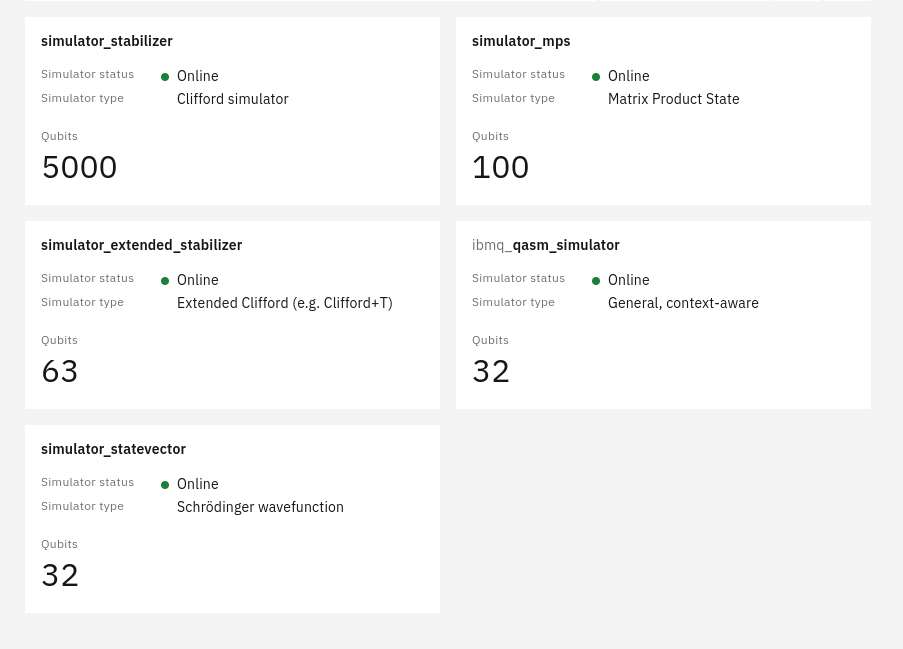
\includegraphics[width=0.9\textwidth]{figures/simulation_services.png}
\caption{Verf\"ugbare Simulatoren bei IBM Quantum}
\label{fig:simulated-services}
\end{figure}
